\documentclass[11pt,twoside,a4paper]{article}
\usepackage[english]{babel}
\usepackage{amsmath}
\usepackage{amsthm}
\usepackage{amssymb}
\usepackage{caption}

\usepackage[pdfstartview=FitH,pdfpagemode=UseNone]{hyperref}
\usepackage[letterspace=40]{microtype}

\usepackage{apacite}
\bibliographystyle{apacite}

\usepackage{a4wide,times}
\usepackage{graphicx}
\usepackage{color}
\usepackage[section]{placeins}

\urlstyle{same}
\linespread{1.1}

\title{
  IN4085 Pattern Recognition\\
  Final Project\\
  ``Classification of Handwritten Digits in Different Scenarios''
}

\author{
    Tung Phan, ttphan, 4004868 \and
    Kevin van Nes, kjmvannes, 4020871
}

%A report detailing the design choices you made for both scenarios, including detailed motivation. This report should discuss the following:
%-the choice of representation (by pixels, features or dissimilarities);
%-the actual features or dissimilarity measure used;
%-for each representation, whether feature reduction is possible and, if so, what number of features should be used;
%-for each representation, the optimal classifier and its type, i.e. parametric (nmc, ldc, qdc, fisherc, loglc), non-parametric (knnc, parzenc) or advanced (neural networks, support vector classifiers, one-class classifiers, combining classifiers);
%-the estimated performance of the optimal classifier on novel data.
%-a test of your system on a set of benchmark data withheld from you by the client (see below). For Scenario 1, your system should have lower than 5\% test error; for Scenario 2, your target is 25\% test error

%Note that each choice is expected to be backed up by either evidence or solid reasoning. In the last exercise(s) for each week you have already experimented somewhat with the hand- written digit dataset. However, it is important to question each step as you construct your final digit recognition system, for two reasons:

%Furthermore:
%-Live test
%-Recommendations

\begin{document}

\maketitle

\section{Introduction}
This report concludes the final assignment of the TI4085 Pattern Recognition course. For this assignment, two classifiers had to be constructed for the classification of handwritten digits. One classifier was made for the scenario in which a lot of training data is available, whilst the other classifier was made for the scenario in which very few training data is available.

This report contains the details about the different phases in constructing the classification system, as well as the design choices that were made and why these were made. Furthermore, the system has been ran against a set of benchmark data, about which more information can also be found in this report. After successfully having created the system, it was ran against a so-called `live test', which is a test in which real, self-written data was used to test the system against. Finally, some recommendations will be given to the company that will receive the system.


\section{Preprocessing}
The first phase we went through during this project was the phase in which we preprocessed the data. This was a necessary step, because the data (i.e. the handwritten digits) differed tremendously amongst each other, even within the same class. An example of this would be that a `4' can be written in different ways or that digits would be sheared in various directions. To solve these inequalities, a few steps were taken to normalize the data, as to try to make the data as similar as possible, both inter-class and intra-class.

\subsection{Boxing and resizing}
The first step that was taken to preprocess the data was to normalize all the data objects in terms of their size. In order to do this, the PRTools functions `im\_box' and `im\_resize' were used. We decided to resize the images to 32x32 pixels (total: 1024 pixels), which later turned out to give better results than images of 64x64 pixels and images of 16x16 pixels. This is probably related to the fact that we use the data images' pixels as our features, so that smaller/larger images would have too few or too many features, respectively.

\subsection{Morphology operations} %(closing for filling holes, erosion + dilation for noise removal)\\
After having normalized the size of the digits, we looked at the images and saw that some of them contained noise. There were also digits that looked incomplete, by which we mean that these digits contained holes that were not supposed to be there. These holes can be seen as another form of noise. We investigated how to solve both of these problems and it turned out that morphology operations were the key to these problems, particularly the closing and opening operators \cite{bishnoi2014, jamil2008noise}.

Firstly, we attempted to fill up the small holes in the images using a closing operator combined with a disk-shaped structuring element of size 1. A closing operator is an operator which first performs a dilation and then an erosion operation. The disk shape (which looks like an addition operator) was chosen to deal with the pixel-like structure of the digits.

After the closing operator had run over an image, noise pixels that were not part of the digits themselves were removed by using an opening operator. An opening operator is an operator which first performs an erosion and then a dilation operation, which makes it the opposite of a closing operation. Again, a disk-shaped structuring element of size 1 was used to perform the opening operator.

\subsection{Shearing for normalization of diagonally orientated digits}
The last major step of preprocessing that was taken was the shearing of all diagonally orientated characters. Because of the differences in the handwritings of people that contributed to the NIST database, some digits of the same kind might look very different from each other, just because they are orientated differently (i.e. skewed). The solution that we implemented in our system consists of two steps: firstly, we use the central moments of the image to determine the orientation angle of the image \cite{gonzalez2002digital}. Secondly we used the orientation angle to skew the digits in the right direction using a simple transformation matrix \cite{yamaguchi2003digit}. The orientation angle was determined in the following way:

Firstly, we determined the moments of the image (i.e. the digits). This can be done using the following formula:\newline
\newline
$M_{ij} = \sum_{x}^{} \sum_{y}^{} x^{i}y^{j}I(x,y)$,
\newline\newline
where $I(x,y)$ is the intensity of a pixel (in our case: 0 or 1) at position (x,y).\\
With this formula, the second-order central moments $\mu_{11}$, $\mu_{20}$ and $\mu_{02}$ were determined by using the following formula:
\newline\newline
$\mu_{pq} = \sum_{x}^{} \sum_{y}^{}(x-\bar{x})(y-\bar{y})f(x,y)$,
\newline\newline
where $f(x,y)$ is pixel intensity of the image at position (x,y) and where $\bar{x} = \frac{M_{10}}{M_{00}}$ and $\bar{y} = \frac{M_{01}}{M_{00}}$.\newline\newline
Finally, using the three central moments that were calculated from the previous formula, we were able to find the orientation angle of each digit, which were determined by:
\newline\newline
$\Theta = \frac{1}{2} arctan(\frac{2\mu_{11}^{'}}{\mu_{20}^{'} - \mu_{02}^{'}})$,
\newline\newline
where $\mu_{11}^{'} = \frac{\mu{11}}{\mu{00}}$, $\mu_{20}^{'} = \frac{\mu{20}}{\mu{00}}$ and $\mu_{02}^{'} = \frac{\mu{02}}{\mu{00}}$.
\newline\newline
After having obtained the orientation angles of the images, we were able to skew them to a vertical orientation by using a simple shearing transformation matrix, which we made as follows:
\newline\newline
$\begin{bmatrix}
       1                       & 0           & 0           \\[0.3em]
       sin(0.5\pi - 2\Theta)   & 1           & 0		   \\[0.3em]
       0                       & 0           & 1
\end{bmatrix}$
\newline\newline\newline
The sinus function in this matrix is used because $sin(0.5\pi)$ represents the y-axis, from which $\Theta$ is subtracted to skew the image in the correct angle. The skewed images are anti-aliased by Matlab, so we turn the digits back into binary images using a threshold function. An example of the result of the preprocessing can be seen in Figure \ref{img:preprocced}.

\begin{figure}[h]
  \centering
  \captionsetup{justification=centering}
  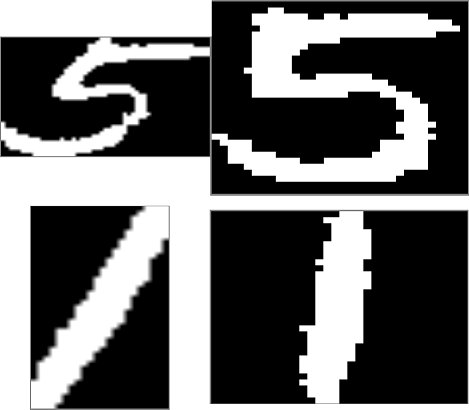
\includegraphics[width=0.5\textwidth]{preprocced.png}
  \caption{Example of preprocessed digits. On the left side, digits are shown before preprocessing. On the right side, the digits have been preprocessed.}
  \label{img:preprocced}
\end{figure}


The combination of the morphological operations and the shearing of the digits resulted in a much better representation of the majority of the digits.\\

\newpage

\section{Feature Extraction}
After the images had all been preprocessed, we wanted to reduce the amount of features in each image (i.e. the pixels). It was found that Principal Component Analysis (PCA) could be used to reduce the amount of features, while keeping as much of the important data as possible. By doing PCA on our images, the most `important' pixels would be retained, while less important pixels would be dismissed.

To hold on to as much of the important data as possible, we did PCA on our data's features with a parameter of 0.99, meaning that 99\% of the total variance of the features would be preserved. As noted earlier, our preprocessed images consist of 1024 pixels each. Our PCA managed to reduce this amount to 625, which means that 399 pixels made up for only 1\% of the total variance of the pixels.


\section{Classifiers}
Now that all of the digit images have been preprocessed and features have been extracted using PCA, the next step was to train the classifiers of our system. Classifiers had to be created for two different scenarios. In the first scenario, Scenario 1, the system is trained once with a large amount of training data, whereas in the second scenario, Scenario 2, the system is trained for each batch of digits, meaning the amount of training data is extremely small.

In the subsections below, the classifiers that we trained for both scenarios will be discussed. Furthermore, the results of what we deemed to be the best classifier for each scenario will be given, based on the classification errors that we calculated for each classifier.
\subsection{Scenario 1}
Scenario 1 is the scenario in which the system is trained with a large amount of training data (at least 200 and at most 1000 objects per class). For such a scenario, it is best to use a classifier that performs well when there is low bias and high variance. Classifiers that we found to be fit for this task were: KNN classfiers and SVM classifiers \cite{liu2003handwritten}. We limited the amount of classifiers in order to save time, as training the classifiers with this amount of training data is very time consuming.

To see which one would be the best fit for our classification, we wrote a function that tested these classifiers simultaneously and it will return the classifier with the lowest error rate. For KNN, we let the K-value be chosen by the implementation, which determined the optimal value with respect to the leave-one-out error. We made use of two different implementations of SVM: rbsvc, which uses a radial basis kernel and cross-validation to determine the best parameters, and libsvc, a more general implementation with the option to specify the kernel to be used. We found out that using a different kernel had an tremendous effect on the performance of the classifier. We tested libsvc utilizing a radial basis kernel, with parameter equal to 7 to 10, and a polynomial type kernel with parameters 2 and 3. We also thought that the Parzen classifier would be a possible candidate, but the parzenc function of PRTools consistently gave back an error rate of 90\% in this scenario, regardless of preprocessing done beforehand. We think it's a bug, so we did not take this result into account.

Table \ref{table:scenario1} shows that SVM with a polynomial basis kernel with parameter 2 performs best, but this is misleading, because radial basis kernel with parameter 10 was more stable, consistently having an error rate lower than 5\%.

\begin{table}[h]
\centering
    \begin{tabular}{ll}
    Classifier                    & Error rate \\ \hline
    KNN                           & 6.95       \\
    SVM (polynomial, parameter 2) & 4.65       \\
    SVM (polynomial, parameter 3) & 4.95       \\
    SVM (radial, parameter 7)     & 6.30       \\
    SVM (radial, parameter 8)     & 5.60       \\
    SVM (radial, parameter 9)     & 5.35       \\
    SVM (radial, parameter 10)    & 4.80       \\
    RBSVM                         & 4.90       \\
    \end{tabular}
    \caption{Results of scenario 1}
    \label{table:scenario1}
\end{table}


\subsection{Scenario 2}
Scenario 2 simulates situations where the classifier is trained before every batch, which means that it has to be fast. As a consequence, the amount of training data is limited with at most 10 objects per class. Using the same setup and preprocessing as with scenario 1, but this time including Parzen, as it performed as expected on small sets of training data. 

We predicted that rbsvc would have the best results thanks to its implemented cross-validation. However, its performance was barely under the 25\% error rate threshold, while radial basis SVM with parameter 10 performed the best. Despite the fact that cross-validation is best suited for small training sets, we think that the set was so small that cross-validation could not sufficiently improve its performance. As can be seen in table \ref{table:scenario2}, radial basis with parameter 7 performs significantly worse and improves by a large margin every time the parameter increases. We thought this trend continued, but curiously, the performance dropped with parameter 11.

\begin{table}[h]
\centering
    \begin{tabular}{ll}
    Classifier                    & Error rate (\%) \\ \hline
    KNN                           & 28.16 \\
    SVM (polynomial, parameter 2) & 24.98           \\
    SVM (polynomial, parameter 3) & 29.10           \\
    SVM (radial, parameter 7)     & 60.30           \\
    SVM (radial, parameter 8)     & 30.30           \\
    SVM (radial, parameter 9)     & 23.66           \\
    SVM (radial, parameter 10)    & \bf{22.20}           \\
    RBSVM                         & 24.32           \\
    Parzen                        & 26.58           \\
    \end{tabular}
    \caption{Results of scenario 2}
    \label{table:scenario2}
\end{table}



\section{Live Test}
After the system was tested against benchmark data, we decided to try and test the system against `live data', which consisted of digits handwritten and scanned in ourself. For each of the digits 0, 1, ..., 9 we wrote six digits each on a piece of paper (see Figure \ref{img:livedata}). After having scanned in the paper, we were able to segment and preprocess the digits to make them ready for classification.

\begin{figure}[h]
  \centering
  \captionsetup{justification=centering}
  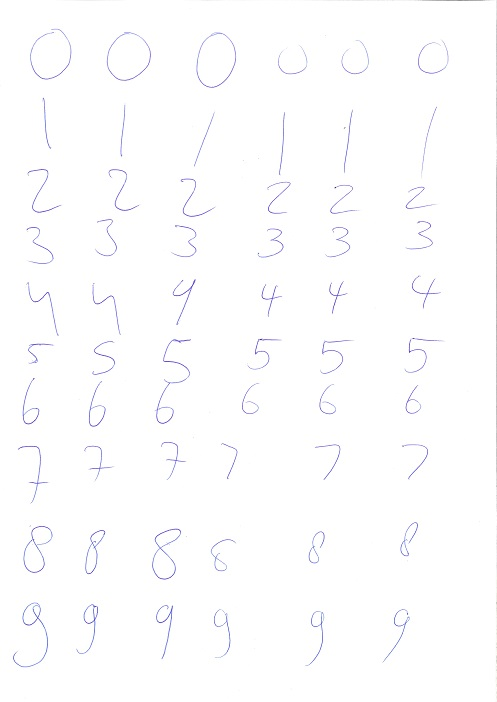
\includegraphics[width=0.5\textwidth]{livedata.jpeg}
  \caption{Live data, handwritten and scanned in ourself}
  \label{img:livedata}
\end{figure}

\subsection{Segmentation and Preprocessing}
Firstly, the 60 handwritten digits were turned into a binary image, after which they were imported into a third-party MATLAB-app, called SegmentTool \cite{segmenttool}. This tool is able to perform segmentation using different kinds of filters and parameters. To segment our digits, we used a Sobel-filter. This was chosen after experimenting manually to retrieve the segmented image that looked best.\newline
\newline
The segmentation resulted in different kinds of noise across the total image containing all digits. These kinds of noise were the same as the kinds of noise that appeared in the original NIST digits. To make sure all images would be cut out correctly in the next step and that no noise would be cut out as if it were a digit, a closing and opening operation were performed on the total image to reduce the noise to a minimum. Next, we cut each digit into its own image by using the MATLAB function \emph{regionprops}. This resulted in each digit being cut out correctly, making them ready for more preprocessing. Since the noise reduction operations have already been applied to the digits, the only preprocessing steps that still had to be taken were the size and orientation normalizations.

\subsection{Classification and Results}
At this point most of the newly handwritten digits look very similar to the digits contained in the database. This means that it was time to use the digits as test data for our classification system. We classified the live test digits using our best classifier for Scenario 1 as well as our best classifier for Scenario 2. 
\newline
\newline
The classifier for Scenario 1 classified our digits with an error rate of 25\%. To reach this rate, we used ???. From our results it could be seen that the classifier had a hard time classifying our '3', '7' and '9' digits. On the other hand, our classifier correctly classified all '1' and '5' digits.\newline
\newline
The classifier for Scenario 2 classified our digits with an error rate of 50\% using the libsvc classifier with radial basis kernel (parameter = 10). We were not satisfied with this result, so we tried running a few other classifiers against our live data to find out that the rbsvc classifier worked slightly better with 43\% error rate. In this case,  \newline
\newline
As can be seen from the results, there is a significant gap between the classification errors of the live tests and that of the benchmark tests. We think that there are several possible reasons for this to have happened.\\
The first possibility is that our preprocessing is not done correctly or exactly in the same way as it is done for the data in the NIST database. It seems that the digits of the NIST database after our preprocessing are much thicker than those of our live data (see Figure \ref{img:thickness}), even though both the NIST data and our live data are preprocessed in the same way. This might be the result of the fact that the digits in the NIST database have been written with a different pen or that they have already been preprocessed slightly by NIST itself.\newline
\begin{figure}[h]
  \centering
  \captionsetup{justification=centering}
  
\includegraphics[width=0.5\textwidth]{NISTvsLIVEthickness.png}
  \caption{Differences in thickness of the digits. The left digit is a preprocessed digit from the NIST database. The right digit is one of our own handwritten digits after the same preprocessing steps.}
  \label{img:thickness}
\end{figure}

We also tried relating the shapes of the digits that were very badly classified during the live test ('3', '7' and '9') to the ones in the database. This showed us that our '7' and '9' digits sometimes deviate a lot from the digits in the database, as can be seen in Figure \ref{img:nistvslive}.\newline
\begin{figure}[h]
  \centering
  \captionsetup{justification=centering}
  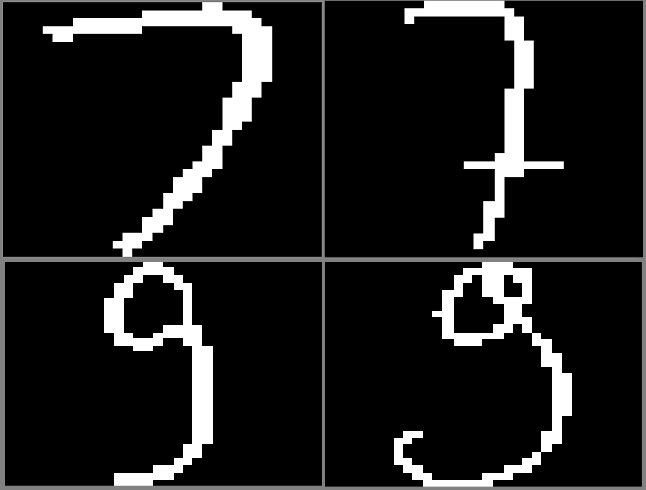
\includegraphics[width=0.5\textwidth]{NISTvsLIVE_7.png}
  \caption{Differences in shapes of digits '7' and '9'. On the left side, the digits from the NIST database are shown, while on the right side the digits from our own handwritten digit set are shown.}
  \label{img:nistvslive}
\end{figure}

The last possibility we came up with as the cause of the disparity between the classification errors is that some of our digits may have been written badly. On the other hand, some of the digits in the NIST database are also incomplete or badly recognizable, so bad writing may not be the reason for higher misclassification at all.

Overall we were satisfied with the results of the live test, as most of the digits (at least in Scenario 1) were recognized correctly and we expect that making some improvements to the preprocessing (and maybe the segmenting) of the self-written digits would improve the classification as well.

\section{Recommendations}
%Recommendations voor bonussssspunt
No handwritten digit recognition system is perfect (although some are getting pretty close \cite{mnist}). This is why in this section some recommendations will be given to suggest possible improvements that could be made to the system in the future.

First off, as we have noticed in the live test, the stroke width of the written numbers have to be of sufficient width. The numbers have to be written with either a marker or preprocessed accordingly to make up for the thin lines. As mentioned earlier, ensuring that the images you train the classifier with and the digits to be read is preprocessed in the same way is crucial. It is possible that the digits provided by NIST are already preprocessed partially, which might have an effect on the performance.

It is also wise to use multiple classifiers to determine the best classifier to be used depending on the error rate. This way, you avoid getting bad results due to outliers (for example, a handwriting that differs a lot from the standard).

We recommend either more training data for scenario 2, in order to make cross-validation feasible, or using the same classifier for every cheque and train it with new numbers every time a cheque is introduced. Doing the latter will ensure that the classifier will receive more training data every time a cheque is presented.

\section{Conclusion}
%Korte conclusie (Nodig?)

\newpage

\bibliography{refs}

\end{document}